
% Default to the notebook output style

    


% Inherit from the specified cell style.




    
\documentclass[11pt]{article}

    
    
    \usepackage[T1]{fontenc}
    % Nicer default font (+ math font) than Computer Modern for most use cases
    \usepackage{mathpazo}

    % Basic figure setup, for now with no caption control since it's done
    % automatically by Pandoc (which extracts ![](path) syntax from Markdown).
    \usepackage{graphicx}
    % We will generate all images so they have a width \maxwidth. This means
    % that they will get their normal width if they fit onto the page, but
    % are scaled down if they would overflow the margins.
    \makeatletter
    \def\maxwidth{\ifdim\Gin@nat@width>\linewidth\linewidth
    \else\Gin@nat@width\fi}
    \makeatother
    \let\Oldincludegraphics\includegraphics
    % Set max figure width to be 80% of text width, for now hardcoded.
    \renewcommand{\includegraphics}[1]{\Oldincludegraphics[width=.8\maxwidth]{#1}}
    % Ensure that by default, figures have no caption (until we provide a
    % proper Figure object with a Caption API and a way to capture that
    % in the conversion process - todo).
    \usepackage{caption}
    \DeclareCaptionLabelFormat{nolabel}{}
    \captionsetup{labelformat=nolabel}

    \usepackage{adjustbox} % Used to constrain images to a maximum size 
    \usepackage{xcolor} % Allow colors to be defined
    \usepackage{enumerate} % Needed for markdown enumerations to work
    \usepackage{geometry} % Used to adjust the document margins
    \usepackage{amsmath} % Equations
    \usepackage{amssymb} % Equations
    \usepackage{textcomp} % defines textquotesingle
    % Hack from http://tex.stackexchange.com/a/47451/13684:
    \AtBeginDocument{%
        \def\PYZsq{\textquotesingle}% Upright quotes in Pygmentized code
    }
    \usepackage{upquote} % Upright quotes for verbatim code
    \usepackage{eurosym} % defines \euro
    \usepackage[mathletters]{ucs} % Extended unicode (utf-8) support
    \usepackage[utf8x]{inputenc} % Allow utf-8 characters in the tex document
    \usepackage{fancyvrb} % verbatim replacement that allows latex
    \usepackage{grffile} % extends the file name processing of package graphics 
                         % to support a larger range 
    % The hyperref package gives us a pdf with properly built
    % internal navigation ('pdf bookmarks' for the table of contents,
    % internal cross-reference links, web links for URLs, etc.)
    \usepackage{hyperref}
    \usepackage{longtable} % longtable support required by pandoc >1.10
    \usepackage{booktabs}  % table support for pandoc > 1.12.2
    \usepackage[inline]{enumitem} % IRkernel/repr support (it uses the enumerate* environment)
    \usepackage[normalem]{ulem} % ulem is needed to support strikethroughs (\sout)
                                % normalem makes italics be italics, not underlines
    

    
    
    % Colors for the hyperref package
    \definecolor{urlcolor}{rgb}{0,.145,.698}
    \definecolor{linkcolor}{rgb}{.71,0.21,0.01}
    \definecolor{citecolor}{rgb}{.12,.54,.11}

    % ANSI colors
    \definecolor{ansi-black}{HTML}{3E424D}
    \definecolor{ansi-black-intense}{HTML}{282C36}
    \definecolor{ansi-red}{HTML}{E75C58}
    \definecolor{ansi-red-intense}{HTML}{B22B31}
    \definecolor{ansi-green}{HTML}{00A250}
    \definecolor{ansi-green-intense}{HTML}{007427}
    \definecolor{ansi-yellow}{HTML}{DDB62B}
    \definecolor{ansi-yellow-intense}{HTML}{B27D12}
    \definecolor{ansi-blue}{HTML}{208FFB}
    \definecolor{ansi-blue-intense}{HTML}{0065CA}
    \definecolor{ansi-magenta}{HTML}{D160C4}
    \definecolor{ansi-magenta-intense}{HTML}{A03196}
    \definecolor{ansi-cyan}{HTML}{60C6C8}
    \definecolor{ansi-cyan-intense}{HTML}{258F8F}
    \definecolor{ansi-white}{HTML}{C5C1B4}
    \definecolor{ansi-white-intense}{HTML}{A1A6B2}

    % commands and environments needed by pandoc snippets
    % extracted from the output of `pandoc -s`
    \providecommand{\tightlist}{%
      \setlength{\itemsep}{0pt}\setlength{\parskip}{0pt}}
    \DefineVerbatimEnvironment{Highlighting}{Verbatim}{commandchars=\\\{\}}
    % Add ',fontsize=\small' for more characters per line
    \newenvironment{Shaded}{}{}
    \newcommand{\KeywordTok}[1]{\textcolor[rgb]{0.00,0.44,0.13}{\textbf{{#1}}}}
    \newcommand{\DataTypeTok}[1]{\textcolor[rgb]{0.56,0.13,0.00}{{#1}}}
    \newcommand{\DecValTok}[1]{\textcolor[rgb]{0.25,0.63,0.44}{{#1}}}
    \newcommand{\BaseNTok}[1]{\textcolor[rgb]{0.25,0.63,0.44}{{#1}}}
    \newcommand{\FloatTok}[1]{\textcolor[rgb]{0.25,0.63,0.44}{{#1}}}
    \newcommand{\CharTok}[1]{\textcolor[rgb]{0.25,0.44,0.63}{{#1}}}
    \newcommand{\StringTok}[1]{\textcolor[rgb]{0.25,0.44,0.63}{{#1}}}
    \newcommand{\CommentTok}[1]{\textcolor[rgb]{0.38,0.63,0.69}{\textit{{#1}}}}
    \newcommand{\OtherTok}[1]{\textcolor[rgb]{0.00,0.44,0.13}{{#1}}}
    \newcommand{\AlertTok}[1]{\textcolor[rgb]{1.00,0.00,0.00}{\textbf{{#1}}}}
    \newcommand{\FunctionTok}[1]{\textcolor[rgb]{0.02,0.16,0.49}{{#1}}}
    \newcommand{\RegionMarkerTok}[1]{{#1}}
    \newcommand{\ErrorTok}[1]{\textcolor[rgb]{1.00,0.00,0.00}{\textbf{{#1}}}}
    \newcommand{\NormalTok}[1]{{#1}}
    
    % Additional commands for more recent versions of Pandoc
    \newcommand{\ConstantTok}[1]{\textcolor[rgb]{0.53,0.00,0.00}{{#1}}}
    \newcommand{\SpecialCharTok}[1]{\textcolor[rgb]{0.25,0.44,0.63}{{#1}}}
    \newcommand{\VerbatimStringTok}[1]{\textcolor[rgb]{0.25,0.44,0.63}{{#1}}}
    \newcommand{\SpecialStringTok}[1]{\textcolor[rgb]{0.73,0.40,0.53}{{#1}}}
    \newcommand{\ImportTok}[1]{{#1}}
    \newcommand{\DocumentationTok}[1]{\textcolor[rgb]{0.73,0.13,0.13}{\textit{{#1}}}}
    \newcommand{\AnnotationTok}[1]{\textcolor[rgb]{0.38,0.63,0.69}{\textbf{\textit{{#1}}}}}
    \newcommand{\CommentVarTok}[1]{\textcolor[rgb]{0.38,0.63,0.69}{\textbf{\textit{{#1}}}}}
    \newcommand{\VariableTok}[1]{\textcolor[rgb]{0.10,0.09,0.49}{{#1}}}
    \newcommand{\ControlFlowTok}[1]{\textcolor[rgb]{0.00,0.44,0.13}{\textbf{{#1}}}}
    \newcommand{\OperatorTok}[1]{\textcolor[rgb]{0.40,0.40,0.40}{{#1}}}
    \newcommand{\BuiltInTok}[1]{{#1}}
    \newcommand{\ExtensionTok}[1]{{#1}}
    \newcommand{\PreprocessorTok}[1]{\textcolor[rgb]{0.74,0.48,0.00}{{#1}}}
    \newcommand{\AttributeTok}[1]{\textcolor[rgb]{0.49,0.56,0.16}{{#1}}}
    \newcommand{\InformationTok}[1]{\textcolor[rgb]{0.38,0.63,0.69}{\textbf{\textit{{#1}}}}}
    \newcommand{\WarningTok}[1]{\textcolor[rgb]{0.38,0.63,0.69}{\textbf{\textit{{#1}}}}}
    
    
    % Define a nice break command that doesn't care if a line doesn't already
    % exist.
    \def\br{\hspace*{\fill} \\* }
    % Math Jax compatability definitions
    \def\gt{>}
    \def\lt{<}
    % Document parameters
    \title{presentation}
    
    
    

    % Pygments definitions
    
\makeatletter
\def\PY@reset{\let\PY@it=\relax \let\PY@bf=\relax%
    \let\PY@ul=\relax \let\PY@tc=\relax%
    \let\PY@bc=\relax \let\PY@ff=\relax}
\def\PY@tok#1{\csname PY@tok@#1\endcsname}
\def\PY@toks#1+{\ifx\relax#1\empty\else%
    \PY@tok{#1}\expandafter\PY@toks\fi}
\def\PY@do#1{\PY@bc{\PY@tc{\PY@ul{%
    \PY@it{\PY@bf{\PY@ff{#1}}}}}}}
\def\PY#1#2{\PY@reset\PY@toks#1+\relax+\PY@do{#2}}

\expandafter\def\csname PY@tok@w\endcsname{\def\PY@tc##1{\textcolor[rgb]{0.73,0.73,0.73}{##1}}}
\expandafter\def\csname PY@tok@c\endcsname{\let\PY@it=\textit\def\PY@tc##1{\textcolor[rgb]{0.25,0.50,0.50}{##1}}}
\expandafter\def\csname PY@tok@cp\endcsname{\def\PY@tc##1{\textcolor[rgb]{0.74,0.48,0.00}{##1}}}
\expandafter\def\csname PY@tok@k\endcsname{\let\PY@bf=\textbf\def\PY@tc##1{\textcolor[rgb]{0.00,0.50,0.00}{##1}}}
\expandafter\def\csname PY@tok@kp\endcsname{\def\PY@tc##1{\textcolor[rgb]{0.00,0.50,0.00}{##1}}}
\expandafter\def\csname PY@tok@kt\endcsname{\def\PY@tc##1{\textcolor[rgb]{0.69,0.00,0.25}{##1}}}
\expandafter\def\csname PY@tok@o\endcsname{\def\PY@tc##1{\textcolor[rgb]{0.40,0.40,0.40}{##1}}}
\expandafter\def\csname PY@tok@ow\endcsname{\let\PY@bf=\textbf\def\PY@tc##1{\textcolor[rgb]{0.67,0.13,1.00}{##1}}}
\expandafter\def\csname PY@tok@nb\endcsname{\def\PY@tc##1{\textcolor[rgb]{0.00,0.50,0.00}{##1}}}
\expandafter\def\csname PY@tok@nf\endcsname{\def\PY@tc##1{\textcolor[rgb]{0.00,0.00,1.00}{##1}}}
\expandafter\def\csname PY@tok@nc\endcsname{\let\PY@bf=\textbf\def\PY@tc##1{\textcolor[rgb]{0.00,0.00,1.00}{##1}}}
\expandafter\def\csname PY@tok@nn\endcsname{\let\PY@bf=\textbf\def\PY@tc##1{\textcolor[rgb]{0.00,0.00,1.00}{##1}}}
\expandafter\def\csname PY@tok@ne\endcsname{\let\PY@bf=\textbf\def\PY@tc##1{\textcolor[rgb]{0.82,0.25,0.23}{##1}}}
\expandafter\def\csname PY@tok@nv\endcsname{\def\PY@tc##1{\textcolor[rgb]{0.10,0.09,0.49}{##1}}}
\expandafter\def\csname PY@tok@no\endcsname{\def\PY@tc##1{\textcolor[rgb]{0.53,0.00,0.00}{##1}}}
\expandafter\def\csname PY@tok@nl\endcsname{\def\PY@tc##1{\textcolor[rgb]{0.63,0.63,0.00}{##1}}}
\expandafter\def\csname PY@tok@ni\endcsname{\let\PY@bf=\textbf\def\PY@tc##1{\textcolor[rgb]{0.60,0.60,0.60}{##1}}}
\expandafter\def\csname PY@tok@na\endcsname{\def\PY@tc##1{\textcolor[rgb]{0.49,0.56,0.16}{##1}}}
\expandafter\def\csname PY@tok@nt\endcsname{\let\PY@bf=\textbf\def\PY@tc##1{\textcolor[rgb]{0.00,0.50,0.00}{##1}}}
\expandafter\def\csname PY@tok@nd\endcsname{\def\PY@tc##1{\textcolor[rgb]{0.67,0.13,1.00}{##1}}}
\expandafter\def\csname PY@tok@s\endcsname{\def\PY@tc##1{\textcolor[rgb]{0.73,0.13,0.13}{##1}}}
\expandafter\def\csname PY@tok@sd\endcsname{\let\PY@it=\textit\def\PY@tc##1{\textcolor[rgb]{0.73,0.13,0.13}{##1}}}
\expandafter\def\csname PY@tok@si\endcsname{\let\PY@bf=\textbf\def\PY@tc##1{\textcolor[rgb]{0.73,0.40,0.53}{##1}}}
\expandafter\def\csname PY@tok@se\endcsname{\let\PY@bf=\textbf\def\PY@tc##1{\textcolor[rgb]{0.73,0.40,0.13}{##1}}}
\expandafter\def\csname PY@tok@sr\endcsname{\def\PY@tc##1{\textcolor[rgb]{0.73,0.40,0.53}{##1}}}
\expandafter\def\csname PY@tok@ss\endcsname{\def\PY@tc##1{\textcolor[rgb]{0.10,0.09,0.49}{##1}}}
\expandafter\def\csname PY@tok@sx\endcsname{\def\PY@tc##1{\textcolor[rgb]{0.00,0.50,0.00}{##1}}}
\expandafter\def\csname PY@tok@m\endcsname{\def\PY@tc##1{\textcolor[rgb]{0.40,0.40,0.40}{##1}}}
\expandafter\def\csname PY@tok@gh\endcsname{\let\PY@bf=\textbf\def\PY@tc##1{\textcolor[rgb]{0.00,0.00,0.50}{##1}}}
\expandafter\def\csname PY@tok@gu\endcsname{\let\PY@bf=\textbf\def\PY@tc##1{\textcolor[rgb]{0.50,0.00,0.50}{##1}}}
\expandafter\def\csname PY@tok@gd\endcsname{\def\PY@tc##1{\textcolor[rgb]{0.63,0.00,0.00}{##1}}}
\expandafter\def\csname PY@tok@gi\endcsname{\def\PY@tc##1{\textcolor[rgb]{0.00,0.63,0.00}{##1}}}
\expandafter\def\csname PY@tok@gr\endcsname{\def\PY@tc##1{\textcolor[rgb]{1.00,0.00,0.00}{##1}}}
\expandafter\def\csname PY@tok@ge\endcsname{\let\PY@it=\textit}
\expandafter\def\csname PY@tok@gs\endcsname{\let\PY@bf=\textbf}
\expandafter\def\csname PY@tok@gp\endcsname{\let\PY@bf=\textbf\def\PY@tc##1{\textcolor[rgb]{0.00,0.00,0.50}{##1}}}
\expandafter\def\csname PY@tok@go\endcsname{\def\PY@tc##1{\textcolor[rgb]{0.53,0.53,0.53}{##1}}}
\expandafter\def\csname PY@tok@gt\endcsname{\def\PY@tc##1{\textcolor[rgb]{0.00,0.27,0.87}{##1}}}
\expandafter\def\csname PY@tok@err\endcsname{\def\PY@bc##1{\setlength{\fboxsep}{0pt}\fcolorbox[rgb]{1.00,0.00,0.00}{1,1,1}{\strut ##1}}}
\expandafter\def\csname PY@tok@kc\endcsname{\let\PY@bf=\textbf\def\PY@tc##1{\textcolor[rgb]{0.00,0.50,0.00}{##1}}}
\expandafter\def\csname PY@tok@kd\endcsname{\let\PY@bf=\textbf\def\PY@tc##1{\textcolor[rgb]{0.00,0.50,0.00}{##1}}}
\expandafter\def\csname PY@tok@kn\endcsname{\let\PY@bf=\textbf\def\PY@tc##1{\textcolor[rgb]{0.00,0.50,0.00}{##1}}}
\expandafter\def\csname PY@tok@kr\endcsname{\let\PY@bf=\textbf\def\PY@tc##1{\textcolor[rgb]{0.00,0.50,0.00}{##1}}}
\expandafter\def\csname PY@tok@bp\endcsname{\def\PY@tc##1{\textcolor[rgb]{0.00,0.50,0.00}{##1}}}
\expandafter\def\csname PY@tok@fm\endcsname{\def\PY@tc##1{\textcolor[rgb]{0.00,0.00,1.00}{##1}}}
\expandafter\def\csname PY@tok@vc\endcsname{\def\PY@tc##1{\textcolor[rgb]{0.10,0.09,0.49}{##1}}}
\expandafter\def\csname PY@tok@vg\endcsname{\def\PY@tc##1{\textcolor[rgb]{0.10,0.09,0.49}{##1}}}
\expandafter\def\csname PY@tok@vi\endcsname{\def\PY@tc##1{\textcolor[rgb]{0.10,0.09,0.49}{##1}}}
\expandafter\def\csname PY@tok@vm\endcsname{\def\PY@tc##1{\textcolor[rgb]{0.10,0.09,0.49}{##1}}}
\expandafter\def\csname PY@tok@sa\endcsname{\def\PY@tc##1{\textcolor[rgb]{0.73,0.13,0.13}{##1}}}
\expandafter\def\csname PY@tok@sb\endcsname{\def\PY@tc##1{\textcolor[rgb]{0.73,0.13,0.13}{##1}}}
\expandafter\def\csname PY@tok@sc\endcsname{\def\PY@tc##1{\textcolor[rgb]{0.73,0.13,0.13}{##1}}}
\expandafter\def\csname PY@tok@dl\endcsname{\def\PY@tc##1{\textcolor[rgb]{0.73,0.13,0.13}{##1}}}
\expandafter\def\csname PY@tok@s2\endcsname{\def\PY@tc##1{\textcolor[rgb]{0.73,0.13,0.13}{##1}}}
\expandafter\def\csname PY@tok@sh\endcsname{\def\PY@tc##1{\textcolor[rgb]{0.73,0.13,0.13}{##1}}}
\expandafter\def\csname PY@tok@s1\endcsname{\def\PY@tc##1{\textcolor[rgb]{0.73,0.13,0.13}{##1}}}
\expandafter\def\csname PY@tok@mb\endcsname{\def\PY@tc##1{\textcolor[rgb]{0.40,0.40,0.40}{##1}}}
\expandafter\def\csname PY@tok@mf\endcsname{\def\PY@tc##1{\textcolor[rgb]{0.40,0.40,0.40}{##1}}}
\expandafter\def\csname PY@tok@mh\endcsname{\def\PY@tc##1{\textcolor[rgb]{0.40,0.40,0.40}{##1}}}
\expandafter\def\csname PY@tok@mi\endcsname{\def\PY@tc##1{\textcolor[rgb]{0.40,0.40,0.40}{##1}}}
\expandafter\def\csname PY@tok@il\endcsname{\def\PY@tc##1{\textcolor[rgb]{0.40,0.40,0.40}{##1}}}
\expandafter\def\csname PY@tok@mo\endcsname{\def\PY@tc##1{\textcolor[rgb]{0.40,0.40,0.40}{##1}}}
\expandafter\def\csname PY@tok@ch\endcsname{\let\PY@it=\textit\def\PY@tc##1{\textcolor[rgb]{0.25,0.50,0.50}{##1}}}
\expandafter\def\csname PY@tok@cm\endcsname{\let\PY@it=\textit\def\PY@tc##1{\textcolor[rgb]{0.25,0.50,0.50}{##1}}}
\expandafter\def\csname PY@tok@cpf\endcsname{\let\PY@it=\textit\def\PY@tc##1{\textcolor[rgb]{0.25,0.50,0.50}{##1}}}
\expandafter\def\csname PY@tok@c1\endcsname{\let\PY@it=\textit\def\PY@tc##1{\textcolor[rgb]{0.25,0.50,0.50}{##1}}}
\expandafter\def\csname PY@tok@cs\endcsname{\let\PY@it=\textit\def\PY@tc##1{\textcolor[rgb]{0.25,0.50,0.50}{##1}}}

\def\PYZbs{\char`\\}
\def\PYZus{\char`\_}
\def\PYZob{\char`\{}
\def\PYZcb{\char`\}}
\def\PYZca{\char`\^}
\def\PYZam{\char`\&}
\def\PYZlt{\char`\<}
\def\PYZgt{\char`\>}
\def\PYZsh{\char`\#}
\def\PYZpc{\char`\%}
\def\PYZdl{\char`\$}
\def\PYZhy{\char`\-}
\def\PYZsq{\char`\'}
\def\PYZdq{\char`\"}
\def\PYZti{\char`\~}
% for compatibility with earlier versions
\def\PYZat{@}
\def\PYZlb{[}
\def\PYZrb{]}
\makeatother


    % Exact colors from NB
    \definecolor{incolor}{rgb}{0.0, 0.0, 0.5}
    \definecolor{outcolor}{rgb}{0.545, 0.0, 0.0}



    
    % Prevent overflowing lines due to hard-to-break entities
    \sloppy 
    % Setup hyperref package
    \hypersetup{
      breaklinks=true,  % so long urls are correctly broken across lines
      colorlinks=true,
      urlcolor=urlcolor,
      linkcolor=linkcolor,
      citecolor=citecolor,
      }
    % Slightly bigger margins than the latex defaults
    
    \geometry{verbose,tmargin=1in,bmargin=1in,lmargin=1in,rmargin=1in}
    
    

    \begin{document}
    
    
    \maketitle
    
    

    
    \begin{Verbatim}[commandchars=\\\{\}]
{\color{incolor}In [{\color{incolor}1}]:} \PY{c+c1}{\PYZsh{}\PYZsh{} Издевательство над текстом в ячейках}
        \PY{k+kn}{from} \PY{n+nn}{IPython}\PY{n+nn}{.}\PY{n+nn}{core}\PY{n+nn}{.}\PY{n+nn}{display} \PY{k}{import} \PY{n}{HTML}
        \PY{n}{HTML}\PY{p}{(}\PY{l+s+s2}{\PYZdq{}\PYZdq{}\PYZdq{}}
        \PY{l+s+s2}{\PYZlt{}style\PYZgt{}}
        
        \PY{l+s+s2}{div.text\PYZus{}cell\PYZus{}render h1 }\PY{l+s+s2}{\PYZob{}}\PY{l+s+s2}{ /* Main titles bigger, centered */}
        \PY{l+s+s2}{font\PYZhy{}size: 2em;}
        \PY{l+s+s2}{line\PYZhy{}height:1.1em;}
        \PY{l+s+s2}{text\PYZhy{}align:center;}
        \PY{l+s+s2}{\PYZcb{}}
        
        \PY{l+s+s2}{div.text\PYZus{}cell\PYZus{}render h4 }\PY{l+s+s2}{\PYZob{}}\PY{l+s+s2}{ /*  Parts names nearer from text */}
        \PY{l+s+s2}{margin\PYZhy{}bottom: \PYZhy{}0.5em;}
        \PY{l+s+s2}{\PYZcb{}}
        
        \PY{l+s+s2}{div.text\PYZus{}cell\PYZus{}render ul}\PY{l+s+s2}{\PYZob{}}\PY{l+s+s2}{ /* Customize text cells */}
        \PY{l+s+s2}{margin\PYZhy{}bottom: \PYZhy{}0.4em;}
        \PY{l+s+s2}{columns: 2;}
        \PY{l+s+s2}{\PYZhy{}webkit\PYZhy{}columns: 2;}
        \PY{l+s+s2}{\PYZhy{}moz\PYZhy{}columns: 2;}
        \PY{l+s+s2}{list\PYZhy{}style\PYZhy{}position: inside;}
        \PY{l+s+s2}{\PYZcb{}}
        \PY{l+s+s2}{div.text\PYZus{}cell\PYZus{}render }\PY{l+s+s2}{\PYZob{}}\PY{l+s+s2}{ /* Customize text cells */}
        \PY{l+s+s2}{font\PYZhy{}size:1.5em;}
        \PY{l+s+s2}{line\PYZhy{}height:1.4em;}
        \PY{l+s+s2}{padding\PYZhy{}left:3em;}
        \PY{l+s+s2}{padding\PYZhy{}right:3em;}
        \PY{l+s+s2}{\PYZcb{}}
        \PY{l+s+s2}{\PYZlt{}/style\PYZgt{}}
        \PY{l+s+s2}{\PYZdq{}\PYZdq{}\PYZdq{}}\PY{p}{)}
\end{Verbatim}


\begin{Verbatim}[commandchars=\\\{\}]
{\color{outcolor}Out[{\color{outcolor}1}]:} <IPython.core.display.HTML object>
\end{Verbatim}
            
    \begin{Verbatim}[commandchars=\\\{\}]
{\color{incolor}In [{\color{incolor}3}]:} \PY{k+kn}{import} \PY{n+nn}{pickle}
        \PY{k+kn}{import} \PY{n+nn}{numpy} \PY{k}{as} \PY{n+nn}{np}
        \PY{k+kn}{import} \PY{n+nn}{pandas} \PY{k}{as} \PY{n+nn}{pd}
        \PY{k+kn}{import} \PY{n+nn}{matplotlib}\PY{n+nn}{.}\PY{n+nn}{pyplot} \PY{k}{as} \PY{n+nn}{plt}
        \PY{o}{\PYZpc{}}\PY{k}{matplotlib} notebook
\end{Verbatim}


    \begin{Verbatim}[commandchars=\\\{\}]
{\color{incolor}In [{\color{incolor}4}]:} \PY{k}{def} \PY{n+nf}{pickle\PYZus{}dump}\PY{p}{(}\PY{n}{obj}\PY{p}{,} \PY{n}{filepath}\PY{p}{)}\PY{p}{:}
            \PY{k}{with} \PY{n+nb}{open}\PY{p}{(}\PY{n}{filepath}\PY{p}{,} \PY{l+s+s1}{\PYZsq{}}\PY{l+s+s1}{wb}\PY{l+s+s1}{\PYZsq{}}\PY{p}{)} \PY{k}{as} \PY{n}{file}\PY{p}{:}
                \PY{n}{pickle}\PY{o}{.}\PY{n}{dump}\PY{p}{(}\PY{n}{obj}\PY{p}{,} \PY{n}{file}\PY{p}{)}
        \PY{k}{def} \PY{n+nf}{pickle\PYZus{}load}\PY{p}{(}\PY{n}{filepath}\PY{p}{)}\PY{p}{:}
            \PY{k}{with} \PY{n+nb}{open}\PY{p}{(}\PY{n}{filepath}\PY{p}{,} \PY{l+s+s1}{\PYZsq{}}\PY{l+s+s1}{rb}\PY{l+s+s1}{\PYZsq{}}\PY{p}{)} \PY{k}{as} \PY{n}{file}\PY{p}{:}
                \PY{n}{res} \PY{o}{=} \PY{n}{pickle}\PY{o}{.}\PY{n}{load}\PY{p}{(}\PY{n}{file}\PY{p}{)}
            \PY{k}{return} \PY{n}{res}
\end{Verbatim}


    \section{Автоматическое извлечение риторических отношений на уровне
предложения в русском
языке}\label{ux430ux432ux442ux43eux43cux430ux442ux438ux447ux435ux441ux43aux43eux435-ux438ux437ux432ux43bux435ux447ux435ux43dux438ux435-ux440ux438ux442ux43eux440ux438ux447ux435ux441ux43aux438ux445-ux43eux442ux43dux43eux448ux435ux43dux438ux439-ux43dux430-ux443ux440ux43eux432ux43dux435-ux43fux440ux435ux434ux43bux43eux436ux435ux43dux438ux44f-ux432-ux440ux443ux441ux441ux43aux43eux43c-ux44fux437ux44bux43aux435}

Захарова Е., БКЛ-142\\
Научный руководитель - Толдова С.Ю.

    \subsection{Информация о дискурсивной структуре может использоваться в
задачах}\label{ux438ux43dux444ux43eux440ux43cux430ux446ux438ux44f-ux43e-ux434ux438ux441ux43aux443ux440ux441ux438ux432ux43dux43eux439-ux441ux442ux440ux443ux43aux442ux443ux440ux435-ux43cux43eux436ux435ux442-ux438ux441ux43fux43eux43bux44cux437ux43eux432ux430ux442ux44cux441ux44f-ux432-ux437ux430ux434ux430ux447ux430ux445}

\begin{itemize}
\tightlist
\item
  извлечения фактов/мнений
\item
  summarization
\item
  анализа тональности
\item
  определения фейковых новостей
\item
  машинного перевода
\item
  автоматической генерации текста
\end{itemize}

    \subsection{Теория Риторических
Структур}\label{ux442ux435ux43eux440ux438ux44f-ux440ux438ux442ux43eux440ux438ux447ux435ux441ux43aux438ux445-ux441ux442ux440ux443ux43aux442ux443ux440}

\begin{itemize}
\tightlist
\item
  формальный анализ дискурсивной структуры текста
\item
  by Mann, Thompson ... 1980-е
\item
  изначально предназначалась для задачи автоматической генерации текста
\item
  сейчас имеет независимый теоретический статус \#\#\# Основные идеи:
\item
  Текст отличается от случайного набора предложений свойствами
  целостности и связности: каждая из частей текста обладает собственной
  функцией
\item
  Части текста на всех уровнях связаны \textbf{риторическими
  отношениями}
\item
  Текст - древовидная структура
\end{itemize}

    \textbf{Элментарная Дискурсивная Единица (ЭДЕ)} - единица дискурса
низшего уровня (квант дискурса), обычно совпадает с клаузой

    \subsection{Риторические
отношения}\label{ux440ux438ux442ux43eux440ux438ux447ux435ux441ux43aux438ux435-ux43eux442ux43dux43eux448ux435ux43dux438ux44f}

\textbf{Асимметричные}: \textbf{Ядро} (Nucleus) - основное значение,
\textbf{Сателлит} (Satellite) - опциональная часть\\
\textbf{Симметричные}: 2 и более \textbf{Ядер} \#\#\#\# Асимметричные: +
Background + Cause-Effect + Evidence + Condition + Purpose + Concession
+ Preparation + Conclusion + Elaboration, + Antithesis + Solutionhood +
Interpretation-Evaluation + Attribution

\paragraph{Симметричные:}\label{ux441ux438ux43cux43cux435ux442ux440ux438ux447ux43dux44bux435}

\begin{itemize}
\tightlist
\item
  Contrast
\item
  Restatement
\item
  Sequence
\item
  Joint
\item
  Comparison
\item
  Same-unit
\end{itemize}

    \subsection{Пример риторической
структуры}\label{ux43fux440ux438ux43cux435ux440-ux440ux438ux442ux43eux440ux438ux447ux435ux441ux43aux43eux439-ux441ux442ux440ux443ux43aux442ux443ux440ux44b}

\begin{figure}
\centering
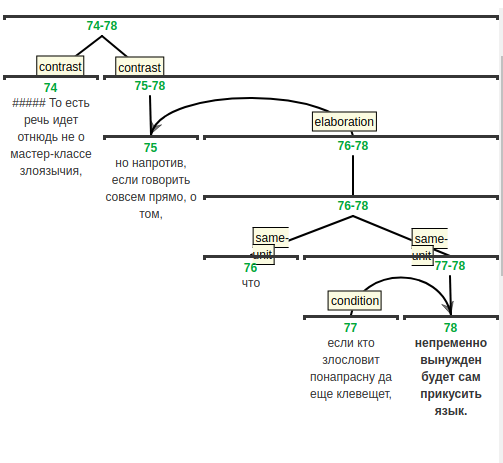
\includegraphics{dt_example.png}
\caption{}
\end{figure}

    \textbf{Дискурсивные маркеры} - сигнализируют присутсвие того или иного
отношения (\emph{если} -\textgreater{} condition и т.д.)

    \subsection{Автоматический анализ
дискурса}\label{ux430ux432ux442ux43eux43cux430ux442ux438ux447ux435ux441ux43aux438ux439-ux430ux43dux430ux43bux438ux437-ux434ux438ux441ux43aux443ux440ux441ux430}

Две подзадачи: сегментация (деление на ЭДЕ), парсинг.\\
Для английского: сегментация - state-of-the-art, парсинг - еще нет.\\
Для русского - вообще ничего. \#\#\#\# Существующие парсеры - идеи: +
Машинное обучение \textless{} правила основанные на маркерах (отношения
без маркеров, не 100\% точные маркеры, неоднозначные маркеры) + Признаки
- лучше группы маркеров или словрь по н-граммам, чем использование
отдельных маркеров + Дискриминативный подход: отдельные алгоритмы для
уровня предложения и уровня текста (разная структура)

    \textbf{Цель} - алгоритм извлечения риторических отношений на уровне
предложения в русских письменных текстах (надеюсь, что в будущем станет
частью полноценного парсера)

    \subsection{Данные}\label{ux434ux430ux43dux43dux44bux435}

Корпус Russian RST Bank (73 текста, \textasciitilde{} по 30
предложений)\\
\textbf{Объекты} - пары ЭДЕ внутри предложения, в рамках окна ширины 5
(4072 объекта)\\
\textbf{Целева переменная} - наличие отношений, тип отношений,
нуклеарность (какая из ЭДЕ - ядро), всего 26 классов (17 отношений)

    \subsection{Распределение
классов}\label{ux440ux430ux441ux43fux440ux435ux434ux435ux43bux435ux43dux438ux435-ux43aux43bux430ux441ux441ux43eux432}

\begin{figure}
\centering
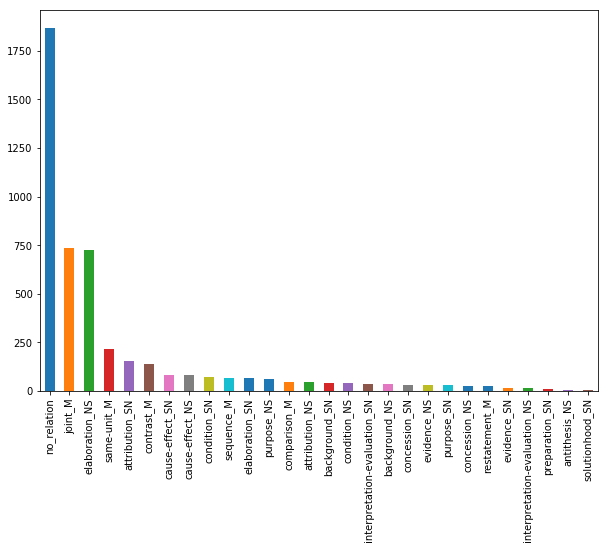
\includegraphics{classes.png}
\caption{}
\end{figure}

    \subsection{Признаки}\label{ux43fux440ux438ux437ux43dux430ux43aux438}

\begin{itemize}
\tightlist
\item
  позиция в тексте
\item
  расстояние (в ЭДЕ)
\item
  длина в токенах
\item
  стоит в начале предложения
\item
  стоит в конце предложения
\item
  количество общих слов (по леммам)
\item
  векторы doc2vec\\
\item
  векторы word2vec первого и последнего токена
\item
  наличие маркера риторических отношений (списки маркеров для каждого из
  отношений, всего Х списков)
\item
  Count Vectorizer по токенам и би- и триграммам токенов (знаки
  препинания учитываются, стоп-слова не удаляются, без лемматизации)
\item
  Count Vectorizer по POS-тегам и би- и триграммам POS-тегов
\end{itemize}

Doc2Vec, Word2Vec - обучение на корпусе серебр. стандарт ГИКРЯ,
Викиновости (без лемматизации, без удаления стоп-слов, знаки препинания
учитывались)

    \subsubsection{Настройка гиперпараметров с помощью Grid
Search}\label{ux43dux430ux441ux442ux440ux43eux439ux43aux430-ux433ux438ux43fux435ux440ux43fux430ux440ux430ux43cux435ux442ux440ux43eux432-ux441-ux43fux43eux43cux43eux449ux44cux44e-grid-search}

    \begin{Verbatim}[commandchars=\\\{\}]
{\color{incolor}In [{\color{incolor}24}]:} \PY{n}{gs}\PY{o}{.}\PY{n}{best\PYZus{}estimator\PYZus{}}
\end{Verbatim}


\begin{Verbatim}[commandchars=\\\{\}]
{\color{outcolor}Out[{\color{outcolor}24}]:} RandomForestClassifier(bootstrap=True, class\_weight=None, criterion='gini',
                     max\_depth=None, max\_features='auto', max\_leaf\_nodes=None,
                     min\_impurity\_decrease=0.0, min\_impurity\_split=None,
                     min\_samples\_leaf=1, min\_samples\_split=2,
                     min\_weight\_fraction\_leaf=0.0, n\_estimators=1500, n\_jobs=3,
                     oob\_score=False, random\_state=669, verbose=0, warm\_start=False)
\end{Verbatim}
            
    \begin{Verbatim}[commandchars=\\\{\}]
{\color{incolor}In [{\color{incolor}5}]:} \PY{c+c1}{\PYZsh{} Display the Dive visualization for this data}
        \PY{k+kn}{from} \PY{n+nn}{IPython}\PY{n+nn}{.}\PY{n+nn}{core}\PY{n+nn}{.}\PY{n+nn}{display} \PY{k}{import} \PY{n}{display}\PY{p}{,} \PY{n}{HTML}
        \PY{n}{data} \PY{o}{=} \PY{n}{pickle\PYZus{}load}\PY{p}{(}\PY{l+s+s1}{\PYZsq{}}\PY{l+s+s1}{data.pkl}\PY{l+s+s1}{\PYZsq{}}\PY{p}{)}
        \PY{n}{features} \PY{o}{=} \PY{n}{data}\PY{o}{.}\PY{n}{columns}
        
        \PY{c+c1}{\PYZsh{} set the sprite\PYZus{}size based on the number of records in dataset,}
        \PY{c+c1}{\PYZsh{} larger datasets can crash the browser if the size is too large (\PYZgt{}50000)}
        \PY{n}{sprite\PYZus{}size} \PY{o}{=} \PY{l+m+mi}{32} \PY{k}{if} \PY{n+nb}{len}\PY{p}{(}\PY{n}{data}\PY{o}{.}\PY{n}{index}\PY{p}{)}\PY{o}{\PYZgt{}}\PY{l+m+mi}{50000} \PY{k}{else} \PY{l+m+mi}{64}
        
        \PY{n}{jsonstr} \PY{o}{=} \PY{n}{data}\PY{o}{.}\PY{n}{to\PYZus{}json}\PY{p}{(}\PY{n}{orient}\PY{o}{=}\PY{l+s+s1}{\PYZsq{}}\PY{l+s+s1}{records}\PY{l+s+s1}{\PYZsq{}}\PY{p}{)}
        \PY{c+c1}{\PYZsh{} Create Facets template  }
        \PY{n}{HTML\PYZus{}TEMPLATE} \PY{o}{=} \PY{l+s+s2}{\PYZdq{}\PYZdq{}\PYZdq{}}\PY{l+s+s2}{\PYZlt{}link rel=}\PY{l+s+s2}{\PYZdq{}}\PY{l+s+s2}{import}\PY{l+s+s2}{\PYZdq{}}\PY{l+s+s2}{ href=}\PY{l+s+s2}{\PYZdq{}}\PY{l+s+s2}{/nbextensions/facets\PYZhy{}dist/facets\PYZhy{}jupyter.html}\PY{l+s+s2}{\PYZdq{}}\PY{l+s+s2}{\PYZgt{}}
        \PY{l+s+s2}{        \PYZlt{}facets\PYZhy{}dive sprite\PYZhy{}image\PYZhy{}width=}\PY{l+s+s2}{\PYZdq{}}\PY{l+s+si}{\PYZob{}sprite\PYZus{}size\PYZcb{}}\PY{l+s+s2}{\PYZdq{}}\PY{l+s+s2}{ sprite\PYZhy{}image\PYZhy{}height=}\PY{l+s+s2}{\PYZdq{}}\PY{l+s+si}{\PYZob{}sprite\PYZus{}size\PYZcb{}}\PY{l+s+s2}{\PYZdq{}}\PY{l+s+s2}{ id=}\PY{l+s+s2}{\PYZdq{}}\PY{l+s+s2}{elem}\PY{l+s+s2}{\PYZdq{}}\PY{l+s+s2}{ height=}\PY{l+s+s2}{\PYZdq{}}\PY{l+s+s2}{650}\PY{l+s+s2}{\PYZdq{}}\PY{l+s+s2}{\PYZgt{}\PYZlt{}/facets\PYZhy{}dive\PYZgt{}}
        \PY{l+s+s2}{        \PYZlt{}script\PYZgt{}}
        \PY{l+s+s2}{          document.querySelector(}\PY{l+s+s2}{\PYZdq{}}\PY{l+s+s2}{\PYZsh{}elem}\PY{l+s+s2}{\PYZdq{}}\PY{l+s+s2}{).data = }\PY{l+s+si}{\PYZob{}jsonstr\PYZcb{}}\PY{l+s+s2}{;}
        \PY{l+s+s2}{        \PYZlt{}/script\PYZgt{}}\PY{l+s+s2}{\PYZdq{}\PYZdq{}\PYZdq{}}
        
        \PY{c+c1}{\PYZsh{} Load the json dataset and the sprite\PYZus{}size into the template}
        \PY{n}{html} \PY{o}{=} \PY{n}{HTML\PYZus{}TEMPLATE}\PY{o}{.}\PY{n}{format}\PY{p}{(}\PY{n}{jsonstr}\PY{o}{=}\PY{n}{jsonstr}\PY{p}{,} \PY{n}{sprite\PYZus{}size}\PY{o}{=}\PY{n}{sprite\PYZus{}size}\PY{p}{)}
\end{Verbatim}


    \subsection{Наиболее важные признаки (первые
150)}\label{ux43dux430ux438ux431ux43eux43bux435ux435-ux432ux430ux436ux43dux44bux435-ux43fux440ux438ux437ux43dux430ux43aux438-ux43fux435ux440ux432ux44bux435-150}

\begin{itemize}
\tightlist
\item
  расстояние между ЭДЕ в паре (в ЭДЕ)
\item
  позиция в тексте (ЭДЕ 1 и 2)
\item
  наличие маркеров condition, наличие "если" (Count Vectorizer)
\item
  наличие маркеров concession, наличие "несмотря" (ЭДЕ 1 и 2)
\item
  наличие маркеров purpose, наличие "чтобы" (ЭДЕ 1 и 2)
\item
  наличие маркеров contrast (ЭДЕ 1 и 2)
\item
  наличие маркеров attribution (ЭДЕ 1 и 2)
\item
  наличие "поскольку" в ЭДЕ 2
\item
  счетчик PRON в ЭДЕ 2
\item
  счетчик NOUN в ЭДЕ 2
\item
  счетчик VERB в ЭДЕ 2
\item
  счетчик CCONJ в ЭДЕ 2
\item
  вектор w2v первого слова ЭДЕ 2
\item
  векоры d2v (ЭДЕ 1 и 2)
\end{itemize}

    \begin{Verbatim}[commandchars=\\\{\}]
{\color{incolor}In [{\color{incolor}6}]:} \PY{c+c1}{\PYZsh{} Display the template}
        \PY{n}{display}\PY{p}{(}\PY{n}{HTML}\PY{p}{(}\PY{n}{html}\PY{p}{)}\PY{p}{)}
\end{Verbatim}


    
    \begin{verbatim}
<IPython.core.display.HTML object>
    \end{verbatim}

    

    % Add a bibliography block to the postdoc
    
    
    
    \end{document}
